\documentclass[11pt]{article}
\usepackage[a4paper,margin=2.3cm]{geometry}
\usepackage[T1]{fontenc}
\usepackage{lmodern}
\usepackage{microtype}
\usepackage{amsmath,amssymb}
\usepackage{booktabs,multirow,makecell,array}
\usepackage[table]{xcolor}
\usepackage{graphicx}
\usepackage{caption}
\usepackage{enumitem}
\usepackage{tikz}
\usetikzlibrary{arrows.meta,positioning,fit,calc}
\usepackage[colorlinks=true,linkcolor=blue!50!black,urlcolor=blue!50!black,citecolor=blue!50!black]{hyperref}
\usepackage{cleveref}
\usepackage{pifont}

\definecolor{okc}{HTML}{2E7D5B}
\definecolor{badc}{HTML}{B3413A}
\definecolor{accent}{HTML}{2F5D8A}
\captionsetup{font=small,labelfont=bf}
\setlist{nosep,leftmargin=*}
\newcommand{\sys}[1]{\textsc{#1}}

\makeatletter\newcommand{\tabinput}[1]{\@@input #1 }\makeatother
% generated by scripts/make_report.py - do not edit
\newcommand{\R}[1]{\ifcsname r@#1\endcsname\csname r@#1\endcsname\else\textbf{??}\fi}
\expandafter\def\csname r@abl-dev_v2_base-acc\endcsname{71.9}
\expandafter\def\csname r@abl-dev_v2_base-hand\endcsname{70.2}
\expandafter\def\csname r@abl-dev_v2_base-recall\endcsname{73.0}
\expandafter\def\csname r@abl-dev_v2_reask-acc\endcsname{75.3}
\expandafter\def\csname r@abl-dev_v2_reask-hand\endcsname{72.1}
\expandafter\def\csname r@abl-dev_v2_reask-recall\endcsname{75.9}
\expandafter\def\csname r@abl-dev_v3_hybrid-acc\endcsname{73.0}
\expandafter\def\csname r@abl-dev_v3_hybrid-hand\endcsname{69.1}
\expandafter\def\csname r@abl-dev_v3_hybrid-recall\endcsname{76.4}
\expandafter\def\csname r@abl-dev_v3_k8-acc\endcsname{75.7}
\expandafter\def\csname r@abl-dev_v3_k8-hand\endcsname{69.8}
\expandafter\def\csname r@abl-dev_v3_k8-recall\endcsname{73.4}
\expandafter\def\csname r@abl-dev_v3_pair-acc\endcsname{71.9}
\expandafter\def\csname r@abl-dev_v3_pair-hand\endcsname{65.0}
\expandafter\def\csname r@abl-dev_v3_pair-recall\endcsname{42.0}
\expandafter\def\csname r@abl-dev_v3_soft-acc\endcsname{73.0}
\expandafter\def\csname r@abl-dev_v3_soft-hand\endcsname{69.5}
\expandafter\def\csname r@abl-dev_v3_soft-recall\endcsname{73.6}
\expandafter\def\csname r@aqua-decision\endcsname{answer}
\expandafter\def\csname r@aqua-gold\endcsname{Jacques Cousteau}
\expandafter\def\csname r@aqua-output\endcsname{Émile Gagnan and Jacques Cousteau}
\expandafter\def\csname r@aqua-planted\endcsname{Bill Nighy}
\expandafter\def\csname r@conf-nli\endcsname{94}
\expandafter\def\csname r@conf-total\endcsname{511}
\expandafter\def\csname r@dev-corpus\endcsname{61{,}500}
\expandafter\def\csname r@dev-leaks\endcsname{638}
\expandafter\def\csname r@dev-n\endcsname{300}
\expandafter\def\csname r@dev-sub-llm\endcsname{72}
\expandafter\def\csname r@dev-sub-pool\endcsname{15}
\expandafter\def\csname r@dev-sub-rule\endcsname{13}
\expandafter\def\csname r@err-total\endcsname{193}
\expandafter\def\csname r@judge-laptop-agree-correct\endcsname{81}
\expandafter\def\csname r@judge-laptop-agree-flagged\endcsname{89}
\expandafter\def\csname r@judge-laptop-agree-handled_ok\endcsname{84}
\expandafter\def\csname r@judge-laptop-agree-misled\endcsname{97}
\expandafter\def\csname r@judge-laptop-pro-acc\endcsname{86.7}
\expandafter\def\csname r@judge-large-agree-correct\endcsname{86}
\expandafter\def\csname r@judge-large-agree-flagged\endcsname{94}
\expandafter\def\csname r@judge-large-agree-handled_ok\endcsname{86}
\expandafter\def\csname r@judge-large-agree-misled\endcsname{98}
\expandafter\def\csname r@judge-large-pro-acc\endcsname{85.1}
\expandafter\def\csname r@laptop-arb-acc\endcsname{68.0}
\expandafter\def\csname r@laptop-arb-balanced_conflict\endcsname{41.5}
\expandafter\def\csname r@laptop-arb-balanced_conflict-flag\endcsname{58.5}
\expandafter\def\csname r@laptop-arb-balanced_conflict-misled\endcsname{12.8}
\expandafter\def\csname r@laptop-arb-f1\endcsname{73.2}
\expandafter\def\csname r@laptop-arb-hand\endcsname{57.0}
\expandafter\def\csname r@laptop-arb-misinfo_majority\endcsname{69.3}
\expandafter\def\csname r@laptop-arb-misinfo_majority-flag\endcsname{66.1}
\expandafter\def\csname r@laptop-arb-misinfo_majority-misled\endcsname{3.2}
\expandafter\def\csname r@laptop-arb-misinfo_single\endcsname{64.1}
\expandafter\def\csname r@laptop-arb-misinfo_single-flag\endcsname{65.2}
\expandafter\def\csname r@laptop-arb-misinfo_single-misled\endcsname{4.3}
\expandafter\def\csname r@laptop-arb-misled\endcsname{2.3}
\expandafter\def\csname r@laptop-arb-no_conflict\endcsname{53.1}
\expandafter\def\csname r@laptop-arb-no_conflict-flag\endcsname{22.4}
\expandafter\def\csname r@laptop-arb-no_conflict-misled\endcsname{0.0}
\expandafter\def\csname r@laptop-arb-p\endcsname{86.8}
\expandafter\def\csname r@laptop-arb-r\endcsname{63.3}
\expandafter\def\csname r@laptop-both-recall\endcsname{74.8}
\expandafter\def\csname r@laptop-ca-acc\endcsname{68.2}
\expandafter\def\csname r@laptop-ca-balanced_conflict\endcsname{40.4}
\expandafter\def\csname r@laptop-ca-balanced_conflict-flag\endcsname{58.5}
\expandafter\def\csname r@laptop-ca-balanced_conflict-misled\endcsname{12.2}
\expandafter\def\csname r@laptop-ca-f1\endcsname{73.2}
\expandafter\def\csname r@laptop-ca-hand\endcsname{56.9}
\expandafter\def\csname r@laptop-ca-misinfo_majority\endcsname{69.3}
\expandafter\def\csname r@laptop-ca-misinfo_majority-flag\endcsname{66.1}
\expandafter\def\csname r@laptop-ca-misinfo_majority-misled\endcsname{3.2}
\expandafter\def\csname r@laptop-ca-misinfo_single\endcsname{64.1}
\expandafter\def\csname r@laptop-ca-misinfo_single-flag\endcsname{65.2}
\expandafter\def\csname r@laptop-ca-misinfo_single-misled\endcsname{4.3}
\expandafter\def\csname r@laptop-ca-misled\endcsname{2.3}
\expandafter\def\csname r@laptop-ca-no_conflict\endcsname{53.6}
\expandafter\def\csname r@laptop-ca-no_conflict-flag\endcsname{22.4}
\expandafter\def\csname r@laptop-ca-no_conflict-misled\endcsname{0.0}
\expandafter\def\csname r@laptop-ca-p\endcsname{86.8}
\expandafter\def\csname r@laptop-ca-r\endcsname{63.3}
\expandafter\def\csname r@laptop-ci-prompted-correct\endcsname{+16.3}
\expandafter\def\csname r@laptop-ci-prompted-handled_ok\endcsname{+22.4}
\expandafter\def\csname r@laptop-ci-prompted-misled\endcsname{-6.3}
\expandafter\def\csname r@laptop-ci-vanilla-correct\endcsname{+13.3}
\expandafter\def\csname r@laptop-ci-vanilla-handled_ok\endcsname{+14.4}
\expandafter\def\csname r@laptop-ci-vanilla-misled\endcsname{-12.6}
\expandafter\def\csname r@laptop-gold-recall\endcsname{79.1}
\expandafter\def\csname r@laptop-minutes\endcsname{30}
\expandafter\def\csname r@laptop-ncomplete\endcsname{791}
\expandafter\def\csname r@laptop-pro-acc\endcsname{51.9}
\expandafter\def\csname r@laptop-pro-balanced_conflict\endcsname{51.1}
\expandafter\def\csname r@laptop-pro-balanced_conflict-flag\endcsname{72.3}
\expandafter\def\csname r@laptop-pro-balanced_conflict-misled\endcsname{6.9}
\expandafter\def\csname r@laptop-pro-f1\endcsname{73.4}
\expandafter\def\csname r@laptop-pro-hand\endcsname{33.5}
\expandafter\def\csname r@laptop-pro-misinfo_majority\endcsname{19.0}
\expandafter\def\csname r@laptop-pro-misinfo_majority-flag\endcsname{69.8}
\expandafter\def\csname r@laptop-pro-misinfo_majority-misled\endcsname{18.0}
\expandafter\def\csname r@laptop-pro-misinfo_single\endcsname{27.2}
\expandafter\def\csname r@laptop-pro-misinfo_single-flag\endcsname{70.1}
\expandafter\def\csname r@laptop-pro-misinfo_single-misled\endcsname{9.8}
\expandafter\def\csname r@laptop-pro-misled\endcsname{8.6}
\expandafter\def\csname r@laptop-pro-no_conflict\endcsname{36.7}
\expandafter\def\csname r@laptop-pro-no_conflict-flag\endcsname{54.1}
\expandafter\def\csname r@laptop-pro-no_conflict-misled\endcsname{0.0}
\expandafter\def\csname r@laptop-pro-p\endcsname{76.2}
\expandafter\def\csname r@laptop-pro-r\endcsname{70.8}
\expandafter\def\csname r@laptop-van-acc\endcsname{54.9}
\expandafter\def\csname r@laptop-van-balanced_conflict\endcsname{0.0}
\expandafter\def\csname r@laptop-van-balanced_conflict-flag\endcsname{0.0}
\expandafter\def\csname r@laptop-van-balanced_conflict-misled\endcsname{13.3}
\expandafter\def\csname r@laptop-van-f1\endcsname{2.8}
\expandafter\def\csname r@laptop-van-hand\endcsname{40.6}
\expandafter\def\csname r@laptop-van-misinfo_majority\endcsname{44.4}
\expandafter\def\csname r@laptop-van-misinfo_majority-flag\endcsname{3.2}
\expandafter\def\csname r@laptop-van-misinfo_majority-misled\endcsname{34.4}
\expandafter\def\csname r@laptop-van-misinfo_single\endcsname{53.8}
\expandafter\def\csname r@laptop-van-misinfo_single-flag\endcsname{1.1}
\expandafter\def\csname r@laptop-van-misinfo_single-misled\endcsname{13.6}
\expandafter\def\csname r@laptop-van-misled\endcsname{14.9}
\expandafter\def\csname r@laptop-van-no_conflict\endcsname{64.3}
\expandafter\def\csname r@laptop-van-no_conflict-flag\endcsname{0.0}
\expandafter\def\csname r@laptop-van-no_conflict-misled\endcsname{0.0}
\expandafter\def\csname r@laptop-van-p\endcsname{--}
\expandafter\def\csname r@laptop-van-r\endcsname{1.4}
\expandafter\def\csname r@laptop-vram\endcsname{4.13}
\expandafter\def\csname r@large-arb-acc\endcsname{76.3}
\expandafter\def\csname r@large-arb-balanced_conflict\endcsname{54.3}
\expandafter\def\csname r@large-arb-balanced_conflict-flag\endcsname{64.9}
\expandafter\def\csname r@large-arb-balanced_conflict-misled\endcsname{8.5}
\expandafter\def\csname r@large-arb-f1\endcsname{75.9}
\expandafter\def\csname r@large-arb-hand\endcsname{67.3}
\expandafter\def\csname r@large-arb-misinfo_majority\endcsname{75.7}
\expandafter\def\csname r@large-arb-misinfo_majority-flag\endcsname{63.0}
\expandafter\def\csname r@large-arb-misinfo_majority-misled\endcsname{3.2}
\expandafter\def\csname r@large-arb-misinfo_single\endcsname{77.7}
\expandafter\def\csname r@large-arb-misinfo_single-flag\endcsname{69.0}
\expandafter\def\csname r@large-arb-misinfo_single-misled\endcsname{2.7}
\expandafter\def\csname r@large-arb-misled\endcsname{1.8}
\expandafter\def\csname r@large-arb-no_conflict\endcsname{61.7}
\expandafter\def\csname r@large-arb-no_conflict-flag\endcsname{17.9}
\expandafter\def\csname r@large-arb-no_conflict-misled\endcsname{0.0}
\expandafter\def\csname r@large-arb-p\endcsname{90.0}
\expandafter\def\csname r@large-arb-r\endcsname{65.6}
\expandafter\def\csname r@large-both-recall\endcsname{74.8}
\expandafter\def\csname r@large-ca-acc\endcsname{76.9}
\expandafter\def\csname r@large-ca-balanced_conflict\endcsname{54.8}
\expandafter\def\csname r@large-ca-balanced_conflict-flag\endcsname{64.9}
\expandafter\def\csname r@large-ca-balanced_conflict-misled\endcsname{8.5}
\expandafter\def\csname r@large-ca-f1\endcsname{75.9}
\expandafter\def\csname r@large-ca-hand\endcsname{67.9}
\expandafter\def\csname r@large-ca-misinfo_majority\endcsname{75.7}
\expandafter\def\csname r@large-ca-misinfo_majority-flag\endcsname{63.0}
\expandafter\def\csname r@large-ca-misinfo_majority-misled\endcsname{3.7}
\expandafter\def\csname r@large-ca-misinfo_single\endcsname{78.3}
\expandafter\def\csname r@large-ca-misinfo_single-flag\endcsname{69.0}
\expandafter\def\csname r@large-ca-misinfo_single-misled\endcsname{2.7}
\expandafter\def\csname r@large-ca-misled\endcsname{2.0}
\expandafter\def\csname r@large-ca-no_conflict\endcsname{62.8}
\expandafter\def\csname r@large-ca-no_conflict-flag\endcsname{17.9}
\expandafter\def\csname r@large-ca-no_conflict-misled\endcsname{0.0}
\expandafter\def\csname r@large-ca-p\endcsname{90.0}
\expandafter\def\csname r@large-ca-r\endcsname{65.6}
\expandafter\def\csname r@large-ci-prompted-correct\endcsname{+1.7}
\expandafter\def\csname r@large-ci-prompted-handled_ok\endcsname{+24.4}
\expandafter\def\csname r@large-ci-prompted-misled\endcsname{-4.3}
\expandafter\def\csname r@large-ci-vanilla-correct\endcsname{+15.1}
\expandafter\def\csname r@large-ci-vanilla-handled_ok\endcsname{+20.2}
\expandafter\def\csname r@large-ci-vanilla-misled\endcsname{-13.3}
\expandafter\def\csname r@large-gold-recall\endcsname{79.1}
\expandafter\def\csname r@large-minutes\endcsname{45}
\expandafter\def\csname r@large-ncomplete\endcsname{791}
\expandafter\def\csname r@large-pro-acc\endcsname{75.3}
\expandafter\def\csname r@large-pro-balanced_conflict\endcsname{51.6}
\expandafter\def\csname r@large-pro-balanced_conflict-flag\endcsname{63.3}
\expandafter\def\csname r@large-pro-balanced_conflict-misled\endcsname{4.3}
\expandafter\def\csname r@large-pro-f1\endcsname{69.9}
\expandafter\def\csname r@large-pro-hand\endcsname{42.3}
\expandafter\def\csname r@large-pro-misinfo_majority\endcsname{30.7}
\expandafter\def\csname r@large-pro-misinfo_majority-flag\endcsname{57.7}
\expandafter\def\csname r@large-pro-misinfo_majority-misled\endcsname{14.3}
\expandafter\def\csname r@large-pro-misinfo_single\endcsname{37.0}
\expandafter\def\csname r@large-pro-misinfo_single-flag\endcsname{63.6}
\expandafter\def\csname r@large-pro-misinfo_single-misled\endcsname{4.9}
\expandafter\def\csname r@large-pro-misled\endcsname{6.3}
\expandafter\def\csname r@large-pro-no_conflict\endcsname{50.0}
\expandafter\def\csname r@large-pro-no_conflict-flag\endcsname{34.7}
\expandafter\def\csname r@large-pro-no_conflict-misled\endcsname{1.0}
\expandafter\def\csname r@large-pro-p\endcsname{81.0}
\expandafter\def\csname r@large-pro-r\endcsname{61.5}
\expandafter\def\csname r@large-van-acc\endcsname{61.9}
\expandafter\def\csname r@large-van-balanced_conflict\endcsname{0.0}
\expandafter\def\csname r@large-van-balanced_conflict-flag\endcsname{0.0}
\expandafter\def\csname r@large-van-balanced_conflict-misled\endcsname{11.2}
\expandafter\def\csname r@large-van-f1\endcsname{0.4}
\expandafter\def\csname r@large-van-hand\endcsname{45.6}
\expandafter\def\csname r@large-van-misinfo_majority\endcsname{46.0}
\expandafter\def\csname r@large-van-misinfo_majority-flag\endcsname{0.5}
\expandafter\def\csname r@large-van-misinfo_majority-misled\endcsname{32.3}
\expandafter\def\csname r@large-van-misinfo_single\endcsname{63.0}
\expandafter\def\csname r@large-van-misinfo_single-flag\endcsname{0.0}
\expandafter\def\csname r@large-van-misinfo_single-misled\endcsname{16.8}
\expandafter\def\csname r@large-van-misled\endcsname{15.3}
\expandafter\def\csname r@large-van-no_conflict\endcsname{73.5}
\expandafter\def\csname r@large-van-no_conflict-flag\endcsname{0.5}
\expandafter\def\csname r@large-van-no_conflict-misled\endcsname{0.0}
\expandafter\def\csname r@large-van-p\endcsname{--}
\expandafter\def\csname r@large-van-r\endcsname{0.2}
\expandafter\def\csname r@large-vram\endcsname{18.56}
\expandafter\def\csname r@match-lenient-ca\endcsname{67.9}
\expandafter\def\csname r@match-lenient-pro\endcsname{42.3}
\expandafter\def\csname r@match-lenient-van\endcsname{45.6}
\expandafter\def\csname r@match-strict-ca\endcsname{65.3}
\expandafter\def\csname r@match-strict-pro\endcsname{40.7}
\expandafter\def\csname r@match-strict-van\endcsname{42.3}
\expandafter\def\csname r@rel-laptop-em\endcsname{55.0}
\expandafter\def\csname r@rel-laptop-prior\endcsname{57.0}
\expandafter\def\csname r@rel-laptop-supervised\endcsname{54.6}
\expandafter\def\csname r@rel-laptop-uniform\endcsname{32.5}
\expandafter\def\csname r@rel-large-em\endcsname{65.2}
\expandafter\def\csname r@rel-large-prior\endcsname{67.3}
\expandafter\def\csname r@rel-large-supervised\endcsname{66.1}
\expandafter\def\csname r@rel-large-uniform\endcsname{42.3}
\expandafter\def\csname r@test-corpus\endcsname{60{,}622}
\expandafter\def\csname r@test-leaks\endcsname{2{,}216}
\expandafter\def\csname r@test-n\endcsname{1000}
\expandafter\def\csname r@test-sub-llm\endcsname{71}
\expandafter\def\csname r@test-sub-pool\endcsname{14}
\expandafter\def\csname r@test-sub-rule\endcsname{15}


\title{\textbf{Conflict-Aware RAG with Evidence Arbitration}\\[2pt]
\large Detecting and arbitrating contradictory evidence in retrieval-augmented generation}
\author{}
\date{November 2026}

\begin{document}
\maketitle

\begin{abstract}
Retrieval-augmented generation (RAG) systems answer from whatever passages they retrieve, so a
single wrong or outdated passage, or a wrong claim repeated by several low-quality sources, can
flip the answer without any warning. We build a RAG system that checks whether retrieved
passages contradict each other before answering. Each passage's answer is extracted as a claim; a
natural-language-inference (NLI) model verifies every claim against its own passage and compares
it with every other passage; verified claims are grouped by stance and weighed by source
reliability. The generator then either answers with the best-supported claim, noting weaker
dissent, or explicitly reports the disagreement. To evaluate it we build a knowledge-conflict
benchmark of \R{test-n} Natural Questions items by editing their gold Wikipedia passages and
mixing them into a \R{test-corpus}-passage corpus. With Qwen2.5-7B, the system handles conflicts
correctly in \R{large-ca-hand}\% of cases (macro average over four scenarios) versus
\R{large-van-hand}\% for standard RAG and \R{large-pro-hand}\% for a RAG baseline explicitly
prompted to handle conflicts, while being misled by planted misinformation in only
\R{large-ca-misled}\% of answerable questions (standard RAG: \R{large-van-misled}\%). The same
pipeline with a 4-bit Qwen2.5-3B, which runs in under 4\,GB of GPU memory, shows the same pattern.
\end{abstract}

\section{Introduction}
Retrieved evidence is not always consistent: encyclopedias are revised, news reports conflict,
and low-quality pages copy each other's mistakes. A standard RAG pipeline concatenates the top
passages and lets the language model resolve any disagreement implicitly, which tends to fail in
two ways: it silently adopts one side (often whichever is repeated more, or appears first), or it
blends incompatible facts.

The project goal is a RAG system that makes the conflict explicit. Concretely:
\begin{enumerate}
  \item detect contradictions between retrieved passages with an NLI model;
  \item group conflicting evidence by stance and weigh it by source reliability;
  \item answer with the best-supported claim, or report the disagreement when no claim is clearly
        better supported;
  \item evaluate on a conflict test set built by editing Wikipedia / Natural Questions passages,
        against standard RAG, on accuracy and conflict-handling quality.
\end{enumerate}

\paragraph{Contributions.} (i) An evidence-arbitration pipeline (claim extraction, NLI
self-verification, stance grouping, reliability-weighted support, a margin-based decision) that
sits between retriever and generator. (ii) A synthetic knowledge-conflict benchmark with four
controlled scenarios over a realistic 60k-passage corpus. (iii) A controlled comparison with
standard and conflict-prompted RAG on two model sizes, with paired bootstrap confidence intervals,
an LLM-judge robustness check, learned source reliability, ablations and an error analysis.
(iv) An interactive web interface that shows the retrieved evidence, the detected conflicts, the
NLI evidence grid, and lets the user change how much each source is trusted.

\section{System}
\begin{figure}[t]
\centering
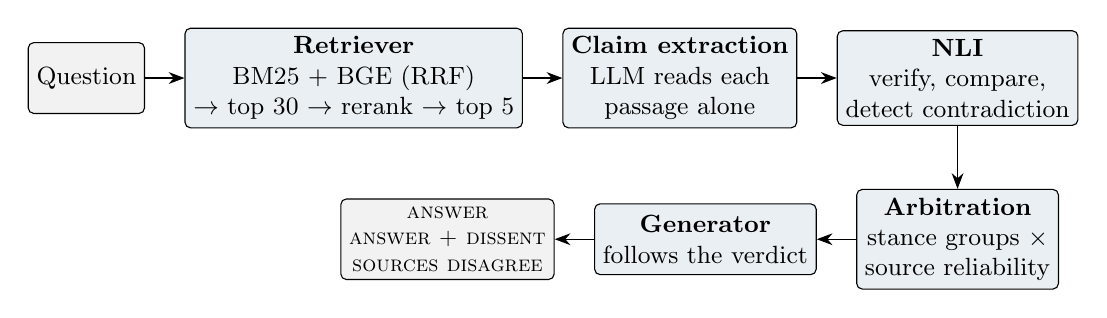
\begin{tikzpicture}[
  node distance=4mm and 5mm,
  box/.style={draw, rounded corners=2pt, align=center, font=\small, minimum height=9mm, inner sep=3pt, fill=#1},
  box/.default=white, >={Stealth[length=2mm]}]
\node[box=gray!10] (q) {Question};
\node[box=accent!10, right=of q] (ret) {\textbf{Retriever}\\BM25 + BGE (RRF)\\$\to$ top 30 $\to$ rerank $\to$ top 5};
\node[box=accent!10, right=of ret] (ext) {\textbf{Claim extraction}\\LLM reads each\\passage alone};
\node[box=accent!10, right=of ext] (nli) {\textbf{NLI}\\verify, compare,\\detect contradiction};
\node[box=accent!10, below=8mm of nli] (arb) {\textbf{Arbitration}\\stance groups $\times$\\source reliability};
\node[box=accent!10, left=of arb] (gen) {\textbf{Generator}\\follows the verdict};
\node[box=gray!10, left=of gen, font=\footnotesize] (out) {\textsc{answer}\\\textsc{answer + dissent}\\\textsc{sources disagree}};
\draw[->] (q) -- (ret); \draw[->] (ret) -- (ext); \draw[->] (ext) -- (nli); \draw[->] (nli) -- (arb);
\draw[->] (arb) -- (gen); \draw[->] (gen) -- (out);
\end{tikzpicture}
\caption{Pipeline. Retrieval, claim extraction and NLI produce per-passage claims with pairwise
entailment/contradiction scores; arbitration turns them into a verdict that the generator follows.}
\label{fig:pipeline}
\end{figure}

\Cref{fig:pipeline} shows the pipeline. All components are open models that run locally.

\subsection{Retriever}
Candidates come from two first-stage retrievers over the same corpus: BM25 (keyword overlap;
$k_1{=}0.9$, $b{=}0.4$) and a dense bi-encoder (\texttt{bge-small-en-v1.5}, cosine similarity of
384-dimensional embeddings, cached on disk). Their top-50 lists are merged by reciprocal rank
fusion, $\mathrm{RRF}(d)=\sum_{r}1/(60+\mathrm{rank}_r(d))$, and a cross-encoder
(\texttt{ms-marco-MiniLM-L-6-v2}) re-scores the top 30 by reading question and passage together.
The best $k{=}5$ are kept; their cross-encoder scores are reused as relevance signals in
arbitration. The correct passage is among the top 5 for \R{large-gold-recall}\% of test
questions.

\subsection{Claim extraction}
The LLM reads each retrieved passage on its own and returns the short answer that passage gives,
or \textsc{none}. Each answer $a_i$ becomes a question-conditioned hypothesis
$h_i=$ ``\emph{The answer to the question ``$q$'' is $a_i$.}'' If the extractor returns \textsc{none}
for a passage whose relevance is within one logit of the best passage, it is asked once more with a
softer prompt (``what answer does this document give?'').

\subsection{NLI verification and comparison}
An NLI cross-encoder (DeBERTa-v3, trained on MNLI/FEVER/ANLI) scores every passage $p_j$ against
every hypothesis $h_i$, giving $E_{ji}=P(p_j\models h_i)$ and $C_{ji}=P(p_j\perp h_i)$.
\begin{itemize}
  \item \textbf{Self-verification:} claim $i$ is kept only if $E_{ii}\ge\tau_v$. This removes answers
        the extractor took from its own memory or from an off-topic passage.
  \item \textbf{Relevance filter:} claims from passages more than 2 reranker logits below the most
        relevant answer-bearing passage are dropped (near-topic passages answering a different
        question).
\end{itemize}

\subsection{Arbitration}
Verified claims with the same normalized answer form a stance group; two groups are merged if NLI
finds them compatible (mean cross-entailment $\ge\tau_e$ and no contradiction $\ge\tau_c$, e.g.\
``1901'' and ``December 10, 1901''). Each group $g$ receives a reliability-weighted noisy-OR support
\begin{equation}
  S(g) = 1-\prod_{j}\bigl(1-r_j\,s_{jg}\bigr),\qquad
  s_{jg}=\begin{cases} E_{jj} & j\in g\\ \tfrac12\max_{i\in g}E_{ji} & j\notin g,\end{cases}
\end{equation}
where $r_j$ is the reliability of passage $j$'s source. Several weak sources add up, but less than
one strong source. Two groups \emph{conflict} if some cross pair has $C\ge\tau_c$, or if they give
distinct verified answers that NLI cannot reconcile. If the top group $g_1$ has a conflicting rival
$g_2$, the decision uses the normalized margin
$\mu=(S(g_1)-S(g_2))/(S(g_1)+S(g_2))$: if $\mu\ge\delta$ the system answers with $g_1$ and mentions
the dissent, otherwise it reports \textsc{sources disagree}. With no verified claim it falls back
to answering from the documents (or ``unknown''). Thresholds ($\tau_v{=}0.3$, $\tau_e{=}\tau_c{=}0.5$,
$\delta{=}0.1$) were chosen by grid search on the development split only.

\subsection{Generation}
The generator receives the passages (with source labels), a short evidence analysis (the
competing claims, their sources and support) and the verdict, with the output format fixed per
verdict, e.g.\ \texttt{ANSWER: Sources disagree: A vs B}. A templated variant that renders the
verdict without the LLM (\sys{arbitration only}) isolates the arbitration module.

\section{Knowledge-conflict benchmark}
\paragraph{Source data.} Natural Questions (NQ-open) questions paired with their gold Wikipedia
passage (\texttt{florin-hf/nq\_open\_gold}; 83k questions, about 64.5k unique passages of
about 105 words).

\paragraph{Counterfactual passages.} For each question whose gold passage contains the answer,
every mention of the answer is replaced by a plausible wrong answer of the same type: years,
dates and numbers are shifted by rule; names and phrases are proposed by Qwen2.5-7B (``a plausible
but incorrect answer of the same kind''), with rejected proposals replaced by another NQ answer to a
question of the same type. Of the test substitutes, \R{test-sub-llm}\% come from the LLM,
\R{test-sub-rule}\% from rules and \R{test-sub-pool}\% from the fallback.

\paragraph{Scenarios and sources.} Each item is assigned one scenario (equal shares):
\begin{center}\small
\begin{tabular}{lll}
\toprule
Scenario & Passages planted in the corpus & Expected behaviour\\
\midrule
No conflict & gold (high-reliability source) & answer gold, no conflict flag\\
Balanced & gold + edited, same reliability tier & report the disagreement, mention both\\
Misinfo $\times1$ & gold (high) + 1 edited (low) & answer gold\\
Misinfo $\times2$ & gold (high) + 2 edited (low) & answer gold (reliability beats majority)\\
\bottomrule
\end{tabular}
\end{center}
{\sloppy High-reliability labels are \texttt{wikipedia}, \texttt{britannica}, \texttt{reuters},
\texttt{bbc} (0.85--0.90); low ones are \texttt{personal-blog}, \texttt{forum}, \texttt{social-media},
\texttt{content-farm} (0.20--0.35). These are synthetic labels: all text is Wikipedia.\par}

\paragraph{Corpus.} The planted passages are mixed with the gold passages of all other NQ questions,
labeled \texttt{wikipedia}, giving \R{test-corpus} passages. Background passages that a benchmark
question retrieves and that state its gold or planted answer (\R{test-leaks}) are removed so that
each scenario contains only its labeled evidence. Retrieval, not the dataset, decides what each
system sees.

\paragraph{Splits.} Test: \R{test-n} questions from the NQ test split. Development:
\R{dev-n} questions from the NQ validation split, with its own corpus, used for all tuning and
ablations.

\section{Experimental setup}
\paragraph{Systems.} All four share the same retrieved passages per question.
\sys{Standard RAG}: top-5 passages $\to$ LLM. \sys{Prompted RAG}: the same plus source labels and
explicit instructions to weigh reliability and report unresolved conflicts (a prompting-only
baseline). \sys{Conflict-aware}: the full pipeline. \sys{Arbitration only}: the verdict rendered by
a template.

\paragraph{Models.} \emph{Large}: Qwen2.5-7B-Instruct (generator and extractor),
DeBERTa-v3-large NLI; peak \R{large-vram}\,GB GPU memory. \emph{Laptop}: Qwen2.5-3B-Instruct in
4-bit, DeBERTa-v3-base NLI; peak \R{laptop-vram}\,GB in batched evaluation.

\paragraph{Metrics.} Scores cover the \R{large-ncomplete} test questions whose gold passage was
retrieved; expected behaviour follows the evidence the system actually saw (if the edited passage
was not retrieved, the no-conflict expectation applies).
\emph{Accuracy}: the gold answer is in the \texttt{ANSWER} line (answerable cases).
\emph{Misled}: the planted answer is given instead of the gold one.
\emph{Handling success}: the scenario's expected behaviour from the table above, macro-averaged
over the four scenarios.
\emph{Conflict detection}: whether the system flags a conflict, against ``gold and edited passage
both retrieved''.
Answers are matched up to wording (``Copernicus'' matches ``Copernicus of Poland''); exact-string
matching gives the same ranking but rejects many correct ``Sources disagree'' answers
(\cref{sec:robustness}).

\section{Results}
\begin{table}[t]
\centering\small
\caption{Test results (\R{test-n} questions; scores on the \R{large-ncomplete} with the gold passage
retrieved). Handling = macro average of scenario-specific success over the four scenarios.}
\label{tab:main}
\begin{tabular}{lcccccc}
\toprule
System & Accuracy & Misled $\downarrow$ & Handling & \multicolumn{3}{c}{Conflict detection}\\
\cmidrule(lr){5-7}
 & & & & P & R & F1\\
\tabinput{generated/table_main.tex}
\bottomrule
\end{tabular}
\end{table}

\begin{table}[t]
\centering\small
\caption{Handling success by scenario (large / laptop).}
\label{tab:scenarios}
\begin{tabular}{lcccc}
\toprule
System & No conflict & Balanced & Misinfo $\times1$ & Misinfo $\times2$\\
\midrule
\tabinput{generated/table_scenarios.tex}
\bottomrule
\end{tabular}
\end{table}

\begin{table}[t]
\centering\small
\caption{Paired bootstrap (2{,}000 resamples), conflict-aware minus baseline, in points, with 95\%
intervals. $^{\dagger}$: interval includes zero.}
\label{tab:ci}
\begin{tabular}{llccc}
\toprule
Profile & Comparison & Handling & Accuracy & Misled\\
\midrule
\tabinput{generated/table_ci.tex}
\bottomrule
\end{tabular}
\end{table}

\Cref{tab:main,tab:scenarios,tab:ci} give the main results.

\paragraph{Arbitration removes most misinformation-driven errors.} When the wrong answer is planted
in low-reliability sources, standard RAG adopts it in \R{large-van-misinfo_majority-misled}\% of
the two-copy cases (large profile); the conflict-aware system does so in
\R{large-ca-misinfo_majority-misled}\%, and handles \R{large-ca-misinfo_majority}\% of these cases
correctly against \R{large-van-misinfo_majority}\% for standard RAG.

\paragraph{Prompting alone is not enough.} Told to weigh reliability and report conflicts, the LLM
flags a conflict on \R{large-pro-no_conflict-flag}\% of questions that have none (conflict-aware:
\R{large-ca-no_conflict-flag}\%) and is still swayed by a misinformation majority. Its overall
handling (\R{large-pro-hand}) is no better than standard RAG (\R{large-van-hand}); the
conflict-aware system improves on it by \R{large-ci-prompted-handled_ok} points.

\paragraph{Accuracy.} With the 7B model, conflict-aware and prompted RAG are close in accuracy
(\R{large-ca-acc} vs \R{large-pro-acc}); both are well above standard RAG (\R{large-van-acc}). With
the 3B model, prompting hurts and the arbitration pipeline is \R{laptop-ci-prompted-correct} points
more accurate than the prompted baseline: an explicit evidence analysis matters more when the
generator is small.

\paragraph{Where it is weaker.} With nothing to arbitrate, standard RAG handles no-conflict
questions best (\R{large-van-no_conflict} vs \R{large-ca-no_conflict}): background passages that
legitimately give a different answer to an ambiguous NQ question are sometimes reported as a
conflict. Balanced conflicts are handled \R{large-ca-balanced_conflict}\% of the time, close to the
prompted baseline (\R{large-pro-balanced_conflict}\%).

\paragraph{The LLM writer adds little.} \sys{Arbitration only} reaches \R{large-arb-hand} handling
against \R{large-ca-hand} for the full system: the gains come from the claim--NLI--arbitration
stages, and the LLM mainly makes the answer readable.

\section{Analysis}

\subsection{How a conflict is resolved: an example}
\begin{table}[t]
\centering\small
\caption{NLI evidence grid for ``\emph{who is given credit for inventing the aqua lung}''
(misinfo~$\times2$; gold: \R{aqua-gold}; planted: \R{aqua-planted}). Cell $(j,i)$: whether passage $j$
supports (\checkmark) or contradicts ($\times$) the claim extracted from passage $i$; bold cells are
self-verification. Output: \emph{\R{aqua-output}}.}
\label{tab:grid}
\resizebox{\linewidth}{!}{\begin{tabular}{lccc}
\toprule
Passage (source) & \makecell{claim of [1]\\\small Émile Gagnan and Jacques Cou} & \makecell{claim of [2]\\\small Bill Nighy and Naval Lieuten} & \makecell{claim of [3]\\\small Bill Nighy and Naval Lieuten} \\
\midrule
{[1]} wikipedia & \textbf{\cellcolor{okc!54}\checkmark\,0.99} & \cellcolor{badc!54}$\times$\,1.00 & \cellcolor{badc!54}$\times$\,1.00 \\
{[2]} personal-blog & \cellcolor{badc!54}$\times$\,0.99 & \textbf{\cellcolor{okc!54}\checkmark\,0.98} & \cellcolor{okc!54}\checkmark\,0.98 \\
{[3]} content-farm & \cellcolor{badc!54}$\times$\,0.99 & \cellcolor{okc!54}\checkmark\,0.98 & \textbf{\cellcolor{okc!54}\checkmark\,0.98} \\
{[4]} wikipedia & \cellcolor{badc!32}$\times$\,0.49 & \cellcolor{badc!32}$\times$\,0.51 & \cellcolor{badc!32}$\times$\,0.51 \\
{[5]} wikipedia & \cellcolor{badc!0}$\times$\,0.05 & \cellcolor{badc!0}$\times$\,0.08 & \cellcolor{badc!0}$\times$\,0.08 \\
\bottomrule
\end{tabular}
}
\end{table}
\Cref{tab:grid} shows the evidence for one test question. The Wikipedia passage and the two
planted low-reliability passages each verify their own claim and contradict the other side;
the reliability-weighted support of the Wikipedia claim exceeds that of the two weak sources
combined, so the system answers with it and mentions the dissenting claim. Over the test set,
the top claim had a counted rival in \R{conf-total} questions; \R{conf-nli}\% of these were direct
NLI contradictions, the rest distinct answers that NLI could not reconcile.

\subsection{Learned source reliability}
\begin{table}[t]
\centering\small
\caption{Re-arbitrating the test evidence with different reliability tables (templated output):
handling / misled / misinfo-$\times2$ handling. Learned tables are fitted on the development split.}
\label{tab:rel}
\begin{tabular}{lcccccc}
\toprule
 & \multicolumn{3}{c}{Large} & \multicolumn{3}{c}{Laptop}\\
\cmidrule(lr){2-4}\cmidrule(lr){5-7}
Reliability table & Hand. & Misled & Misinfo$\times2$ & Hand. & Misled & Misinfo$\times2$\\
\midrule
\tabinput{generated/table_reliability.tex}
\bottomrule
\end{tabular}
\end{table}
The reliability table need not be hand-set. A \emph{supervised} estimate takes, per source, the
smoothed fraction of its claims that agree with the known answer on the development split; an
\emph{EM} estimate (truth discovery) alternates between inferring which stance is true and how often
each source is right, without labels. \Cref{tab:rel} shows that both stay within about three points
of the hand-set table on overall handling, but lose ground on the two-copy misinformation case
(7--13 points), where the outcome depends most on the exact reliability gap. Ignoring reliability
altogether collapses performance on misinformation. Learned values are listed in \cref{app:hyper}. The supervised table gives \texttt{wikipedia} only 0.37: most Wikipedia-labeled passages are background passages that answer a different question, so their claims count as disagreeing with the label. This likely explains much of its loss against two planted copies. Because benchmark sources come from the same synthetic
generator, this shows that the estimators recover planted reliabilities, not that they would score
real web sources well.

\subsection{Robustness of the evaluation}\label{sec:robustness}
\paragraph{Answer matching.} With exact-string matching the large-profile handling scores are
\R{match-strict-ca} (conflict-aware), \R{match-strict-pro} (prompted) and \R{match-strict-van}
(standard), against \R{match-lenient-ca}, \R{match-lenient-pro} and \R{match-lenient-van} with
wording-tolerant matching: the ranking is unchanged.

\paragraph{LLM judge.}
\begin{table}[t]
\centering\small
\caption{Handling success graded by an LLM judge (Qwen2.5-7B) vs.\ the string-matching metric.}
\label{tab:judge}
\begin{tabular}{lcccc}
\toprule
 & \multicolumn{2}{c}{Large} & \multicolumn{2}{c}{Laptop}\\
\cmidrule(lr){2-3}\cmidrule(lr){4-5}
System & Judge & String & Judge & String\\
\midrule
\tabinput{generated/table_judge.tex}
\bottomrule
\end{tabular}
\end{table}
An LLM judge classified each output (gold answer, planted answer, ``sources disagree'' with both,
or other) and re-applied the same handling rules (\cref{tab:judge}). It agrees with string
matching on \R{judge-large-agree-misled}\% of ``misled'' labels and
\R{judge-large-agree-flagged}\% of ``flagged'' labels, and gives the same ranking. It is, however,
not a better metric: in a manual check of disagreements it accepted almost any ``Sources disagree:
X vs Y'' as presenting both answers and missed plain correct answers, inflating the prompted
baseline's judged accuracy (\R{judge-large-pro-acc}\%). The judge is also the generating model.
String matching therefore remains the primary metric.

\subsection{Ablations (development split)}
\begin{table}[t]
\centering\small
\caption{Ablations on the development split (large profile, templated output, \R{dev-n} questions).}
\label{tab:abl}
\begin{tabular}{lccccc}
\toprule
Variant & Gold@5 & Accuracy & Handling & Conflict recall & Balanced\\
\midrule
\tabinput{generated/table_ablations.tex}
\bottomrule
\end{tabular}
\end{table}
\Cref{tab:abl} lists the variants tried on the development split. Re-asking the extractor for
highly relevant passages where it found no answer is the only change kept. Two variants that use
the LLM to judge passages failed in an instructive way. Both an LLM ``scope check'' (does this
passage answer exactly the question?) and a pairwise ``same-subject check'' (are these two
passages about the same thing?) fixed near-miss cases such as ``father of the \emph{personal}
computer'' versus ``father of the computer'', but cut conflict recall sharply: the model rejected
planted passages it believed were false, i.e.\ it replaced the evidence with its own beliefs, which
is exactly what a conflict-aware system must avoid. More passages ($k{=}8$) raise retrieval recall
but add distractors that cost more than they gain.

\subsection{Where conflicts are lost}
\begin{table}[t]
\centering\small
\caption{Why a conflict that was in the retrieved context was not flagged (conflict-aware, large
profile, \R{err-total} cases).}
\label{tab:err}
\begin{tabular}{lcc}
\toprule
First stage that lost the conflict & Cases & Share (\%)\\
\midrule
\tabinput{generated/table_errors.tex}
\bottomrule
\end{tabular}
\end{table}
\Cref{tab:err} attributes missed conflicts to the first stage that lost them. Most losses occur
before arbitration, in claim extraction: the extractor returns no answer, or a different span, for
a passage that does state the answer. Stronger, context-faithful extraction is therefore the most
promising direction.

\section{Interactive interface}
\begin{figure}[t]
\centering
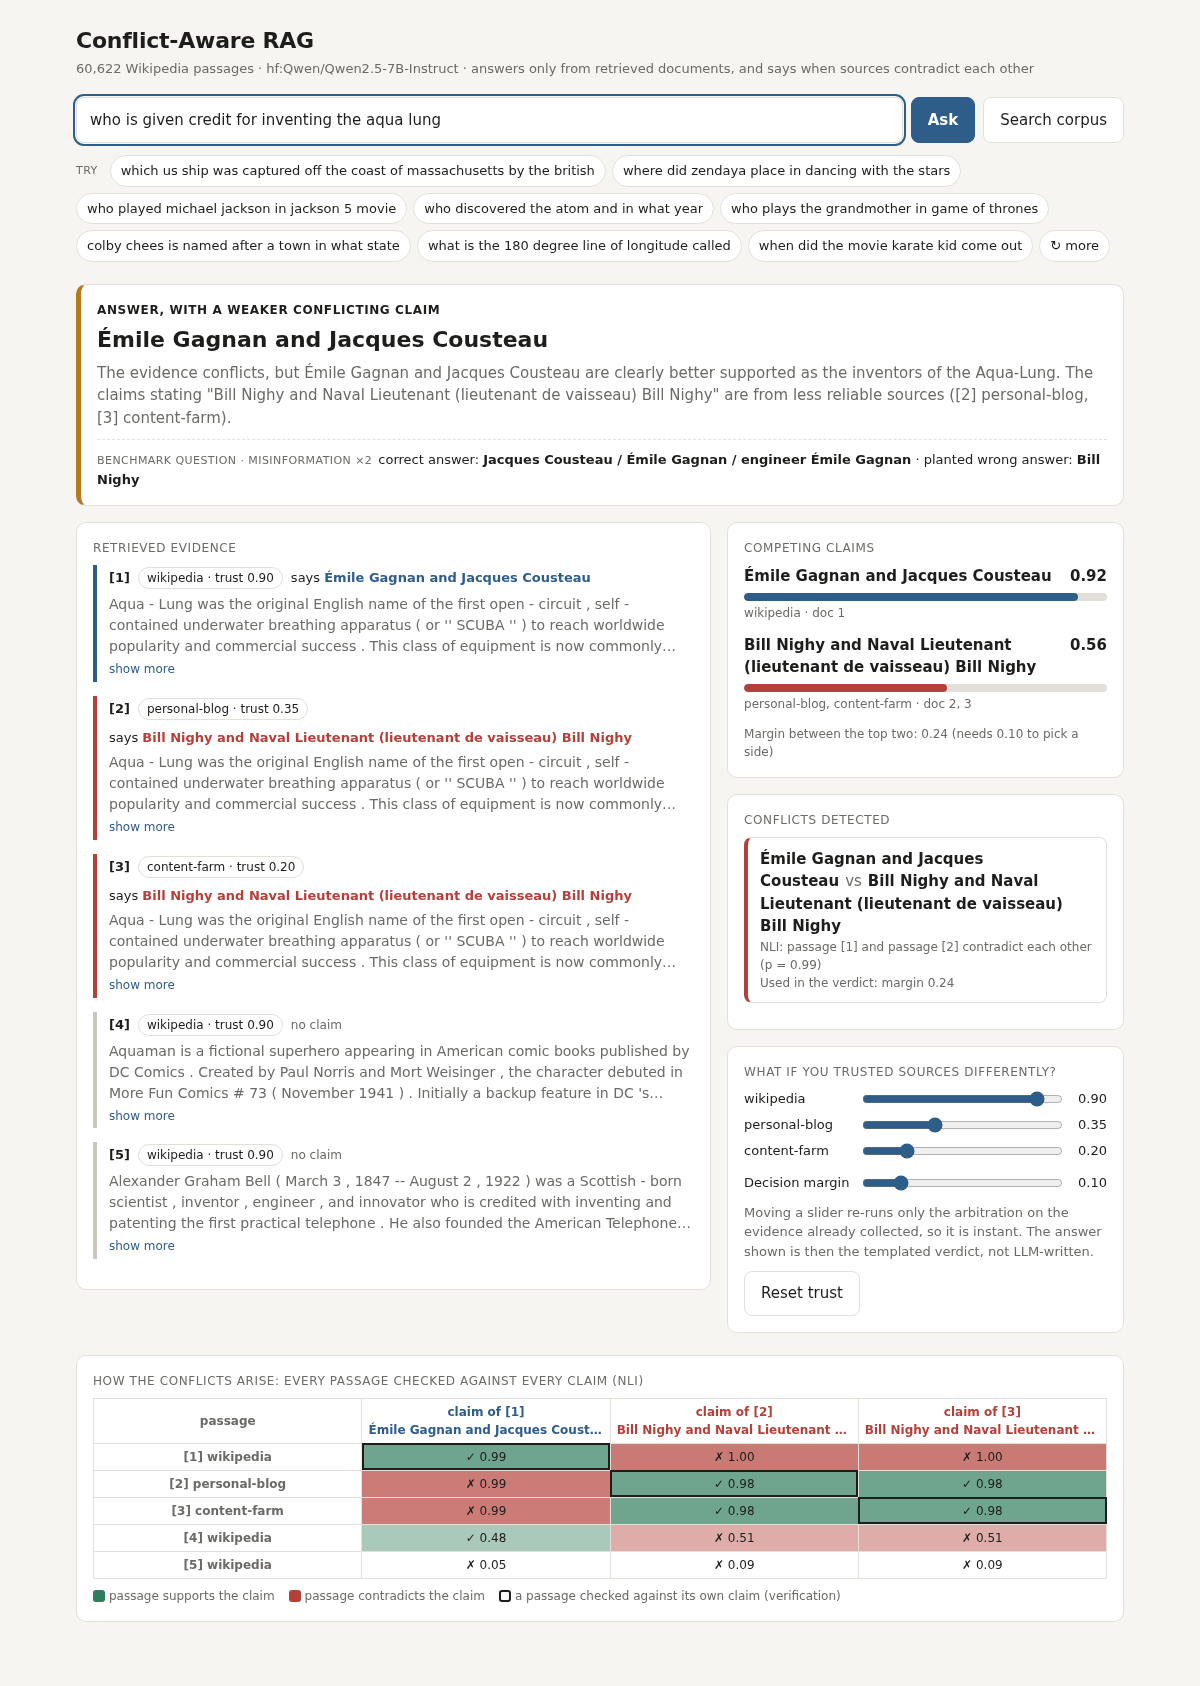
\includegraphics[width=\linewidth]{figures/ui_aqua.png}
\caption{Web interface (\texttt{carag serve}) for the example of \cref{tab:grid}: verdict with the
benchmark's gold and planted answers, retrieved evidence coloured by stance, competing claims with
their support, detected conflicts with reasons, trust sliders, and the NLI evidence grid.}
\label{fig:ui}
\end{figure}
A local web interface (\cref{fig:ui}) exposes every stage: the retrieved passages with source,
trust and extracted claim; the competing claims and their support; each detected conflict with its
reason and whether it decided the verdict; and the passage-by-claim NLI grid. Sliders change the
trust in each source and the decision margin; since only the arbitration is re-run on the
evidence already collected, the verdict updates instantly. The system also runs as a terminal chat
and a command-line tool.

\section{Limitations}
\begin{itemize}
  \item \textbf{Synthetic conflicts.} Conflicts come from entity substitution, so planted passages
        are near-duplicates of the gold ones and tend to be retrieved together; natural conflicts
        (paraphrased, outdated, partially overlapping) are harder.
  \item \textbf{Synthetic reliability.} Source labels and scores are assigned by the benchmark, so the
        reliability signal is informative by construction.
  \item \textbf{Ambiguous questions.} Some NQ questions have several valid answers; flagging those
        counts as a false alarm.
  \item \textbf{Coverage.} The corpus contains only NQ's Wikipedia passages; questions outside it
        cannot be answered from evidence.
  \item \textbf{Near-miss claims.} NLI accepts ``father of the personal computer'' as
        ``father of the computer''; such cases are reported as a disagreement rather than resolved.
  \item \textbf{Hardware.} The laptop profile was measured under a memory cap on a larger GPU, not on
        a physical 4\,GB card or Apple-silicon laptop.
\end{itemize}

\section{Conclusion}
Making conflicts explicit, by extracting each passage's claim, verifying and comparing claims with
NLI, and arbitrating by stance and source reliability, substantially improves how a RAG system
handles contradictory evidence. With Qwen2.5-7B, handling success rises by
\R{large-ci-vanilla-handled_ok} points over standard RAG and \R{large-ci-prompted-handled_ok} over
conflict-prompted RAG, and answers taken from planted misinformation drop from
\R{large-van-misled}\% to \R{large-ca-misled}\%, with accuracy on par with the strongest
baseline. The main remaining
bottleneck is claim extraction; and attempts to let the LLM judge the passages showed that the
arbitration must rely on the documents, not on the model's beliefs.

\appendix
\section{Hyperparameters and learned reliabilities}\label{app:hyper}
\begin{center}\small
\begin{tabular}{ll}
\toprule
Retrieval & BM25 ($k_1{=}0.9$, $b{=}0.4$) + \texttt{bge-small-en-v1.5}, RRF ($k{=}60$, depth 50),\\
          & rerank top 30 with \texttt{ms-marco-MiniLM-L-6-v2}, keep $k{=}5$\\
Arbitration & $\tau_v{=}0.3$, $\tau_e{=}\tau_c{=}0.5$, $\delta{=}0.1$, mean-entailment merging, relevance gap 2.0\\
Generation & greedy decoding, at most 160 new tokens\\
Tuning & grid search on the development split only (\texttt{carag sweep})\\
\bottomrule
\end{tabular}

\vspace{1em}
\begin{tabular}{lccc}
\toprule
Source & Hand-set & Supervised (dev) & EM (dev)\\
\midrule
\tabinput{generated/table_reliability_values.tex}
\bottomrule
\end{tabular}
\end{center}

\section{Reproduction}
\begin{small}
\begin{verbatim}
carag build-data --out data/nq_conflict     --split test       --n 1000 --seed 13
carag build-data --out data/nq_conflict_dev --split validation --n 300  --seed 7
carag eval  --data data/nq_conflict --out runs/test_large  --profile large
carag eval  --data data/nq_conflict --out runs/test_laptop --profile laptop --quantize 4bit
carag judge --run runs/test_large;  carag conflicts --run runs/test_large
python scripts/make_report.py && cd report && pdflatex report && pdflatex report
\end{verbatim}
\end{small}

\end{document}
